\documentclass[12pt]{exam}

\newcommand{\course}{MTH 234 Summer 2021}
\newcommand{\qdate}{15.10} %PUT DATE HERE
\newcommand{\quiz}{Group Work} 

    \usepackage[top=1in, bottom=1in, left=.45in, right=.45in]{geometry}
    \usepackage{amsmath,amsthm,amssymb,amstext}
    \usepackage{enumerate,enumitem}
    \usepackage{tikz,float,graphicx}
    \usepackage{microtype}
    \usepackage{bm,tikz}
        \usetikzlibrary{calc,positioning}
    \usepackage{multicol}
    \usepackage{nicematrix}
    \usepackage{cleveref}
    \usepackage[framemethod=tikz]{mdframed}
    \usepackage{graphicx}
    \usepackage[export]{adjustbox}
    
    %\newcommand{\course}{MTH 234 Summer 2021}
    %\newcommand{\qdate}{Equations of lines and planes} %PUT DATE HERE
    %\newcommand{\quiz}{Group Work} 
    
    \newcommand{\R}{\mathbb{R}}
    
    \newcommand{\ba}{\bm{a}}
    \newcommand{\bb}{\bm{b}}
    \newcommand{\bc}{\bm{c}}
    \newcommand{\bi}{\bm{i}}
    \newcommand{\bj}{\bm{j}}
    \newcommand{\bk}{\bm{k}}
    \newcommand{\br}{\bm{r}}
    \newcommand{\bv}{\bm{v}}
    \newcommand{\bu}{\bm{u}}
    \newcommand{\gen}[1]{\left\langle #1 \right\rangle}
    \newcommand{\pd}[2]{\dfrac{\partial #1}{\partial #2}}

\newtheorem*{theorem}{Theorem}
\surroundwithmdframed[]{theorem}

\theoremstyle{definition}
    \newtheorem*{definition}{Definition}
    \surroundwithmdframed[]{definition}
    \newtheorem*{info}{Useful Information}
    \surroundwithmdframed[]{info}
\theoremstyle{remark}
    \newtheorem*{remark}{Remark}
    \surroundwithmdframed[]{remark}
    

%%%%%%%%%%%%%%%%%%%%%%%
% HEADER AND FOOTER
%%%%%%%%%%%%%%%%%%%%%%%
\pagestyle{headandfoot}
\firstpageheadrule
\runningheadrule
\firstpageheader{\course}{\quiz}{\qdate}
\runningheader{\course}{\quiz}{\qdate}
\runningfooter{}{}{}


\usepackage{color}
\shadedsolutions
\definecolor{SolutionColor}{rgb}{0.8,0.9,1}

\usepackage{pgfplots}
    \pgfplotsset{every axis/.append style={
                    axis x line=middle,    % put the x axis in the middle
                    axis y line=middle,    % put the y axis in the middle
                    axis z line=middle,
                    axis line style={<->}, % arrows on the axis
                    xlabel={$x$},          % default put x on x-axis
                    ylabel={$y$},          % default put y on y-axis
                    zlabel={$z$},
                    grid=both,
                    %xtick={-4,...,-1,1,...,3},
                    %ytick={-1,1,}
    }}
    \pgfplotsset{compat=1.17}

\usetikzlibrary{patterns}
\newcommand{\bif}{\quad\iff\quad}

\printanswers
%\noprintanswers

\begin{document}

\section*{\qdate}

%\subsection*{Template}

\begin{info}
    \begin{itemize}
            \item The \textbf{Jacobian} for a tranformation \(T\) given by \(x=x(u,v)\) and \(y=y(u,v)\) is
            \[
                \dfrac{(x,y)}{(x,y)}=
                \left|\begin{NiceMatrix}
                    \pd{x}{u} & \pd{x}{v}\\
                        &\\
                    \pd{y}{u} & \pd{y}{v}
                \end{NiceMatrix}\right| = \pd{x}{u}\cdot\pd{y}{v}-\pd{x}{v}\cdot\pd{y}{u}
            \]
            \item 
            \[
                \iint_{R}f(x,y)~dA=\iint_{S}f(x(u,v),y(u,v))\left|\dfrac{(u,v)}{(u,v)}\right|~du~dv
            \]
    \end{itemize}
\end{info}


\begin{questions}

\question Show that the Jacobian of the transformation \(x=5u-v,y=u+3v\) is \(16\).
\ifprintanswers
        \begin{solution}
            \begin{align*}
              \pd{x}{u}\cdot\pd{y}{v}-\pd{x}{v}\cdot\pd{y}{u} & = \left( 5 \right)  \left(3\right)-\left(-1\right)\left(1\right)\\
              &= 16.
            \end{align*}
        \end{solution}
    \else
        \vfill
    \fi

\question Show that the Jacobian of the transformation \(x=e^{-r}\sin\theta\), \(y=e^r\cos\theta\) is \(\sin^2\theta-\cos^2\theta\).
\ifprintanswers
        \begin{solution}
            \begin{align*}
                \pd{x}{r}\cdot\pd{y}{\theta}-\pd{x}{\theta}\cdot\pd{y}{r} & = \left(-e^{-r}\sin\theta\right)\left(-e^{r}\sin\theta\right)-\left(e^{-r}\cos\theta\right)\left(e^{r}\cos\theta\right)\\
                &= \sin^2\theta-\cos^2\theta.
            \end{align*}
        \end{solution}
    \else
        \vfill
    \fi

\newpage
\question Evaluate \(\iint_R(x-3y)dA\) where \(R\) is the triangular region with vertices \((0,0)\),\((2,1)\), and \((1,2)\) using the transformation \(x=2u+v\), \(y=u+2v\). Make sure you evaluate it in such a way that the answer you get is \(-3\).
\ifprintanswers
        \begin{solution}
            If \(T\) is the transformation \(x=2u+v\) and \(y=u+2v\) we will first find the image of the triangle \(R\). 
            We can find the inverse transformation by combining the above equations,
            \[
                x-2y=2u+v-2\left(u+2v\right) = -3v \quad\Rightarrow\quad v=\frac{1}{3}\left(2y-x\right)
            \]
            and

            \[
                2x-y = 2\left(2u+v\right)-(u+2v)=3u \quad\Rightarrow\quad u=\frac{1}{3}\left(2x-y\right)
            \]

                \(R\) is bounded by the lines 
                    \begin{equation*}
                        \begin{aligned}
                           L1: ~~~ y&=\frac{1}{2}x &~~\text{with}~~0\le x\le 2 \\
                           L2: ~~~ y&=2x &~~\text{with}~~0\le x\le 1 \\
                           L3: ~~~ y&=3-x &~~\text{with}~~1\le x\le2 
                        \end{aligned}
                    \end{equation*}
                Along \(L1\), 
                \[
                    y=\frac{1}{2}x \quad \Rightarrow\quad u+2v=u+\frac{1}{2}v \quad\Rightarrow\quad v=0
                \]
                \(L2\),
                \[
                    y=2x \quad\Rightarrow\quad u+2v=2\left(2u+v\right) \quad\Rightarrow\quad u=0
                \]
                \(L3\),
                    \[
                        y=3-x \quad\Rightarrow\quad u+2v = 3-\left(2u+v\right) \quad\Rightarrow\quad v=1-u
                    \]
                    
            As seen in the image below, for \(0\le u\le 1\), \(0\le v\le 1-u\).

            \begin{center}
            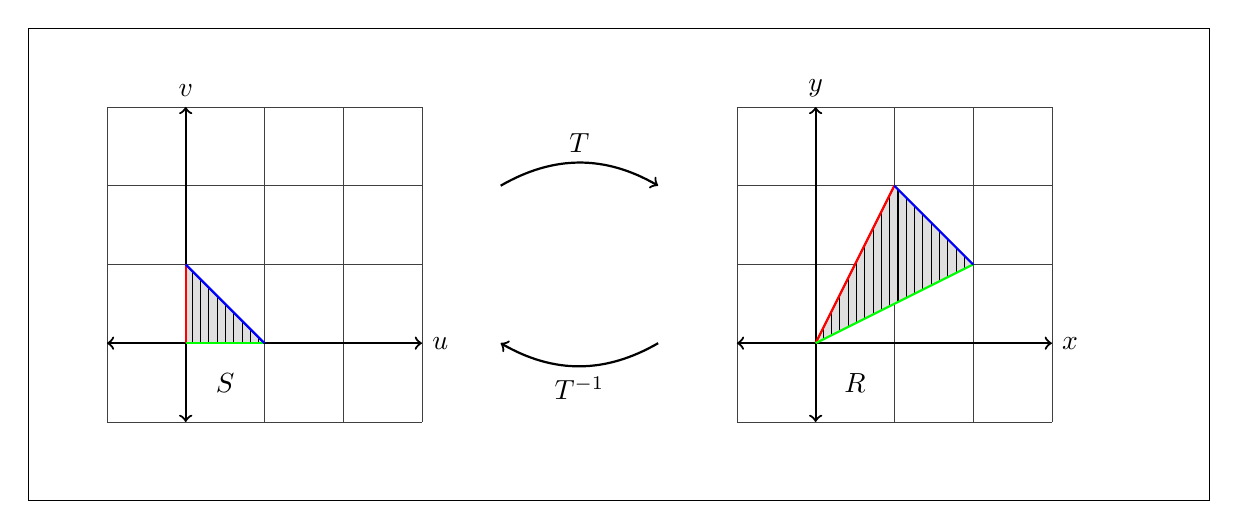
\begin{tikzpicture}
            \draw[fill=white] (-2,-2)--(13,-2)--(13,4)--(-2,4)--(-2,-2);
                \begin{scope}[shift={(8,0)}]
                    
                    \draw[very thin,opacity=.75] (-1,-1) grid (3,3);
                    \draw[<->,thick] (-1,0)--(3,0) node[right] {$x$};
                    \draw[<->,thick] (0,-1)--(0,3) node[above] {$y$};
                        \draw[fill=gray!25!white] (0,0)--(1,2)--(2,1)--(0,0);
                        \draw[pattern=vertical lines] (0,0)--(1,2)--(2,1)--(0,0);
                        \draw[red,thick] (0,0)--(1,2);
                        \draw[green,thick] (0,0)--(2,1);
                        \draw[blue,thick] (1,2)--(2,1);
                    \node at (.5,-.5) {$R$};
                \end{scope}
                \begin{scope}
                    \draw[very thin,opacity=.75] (-1,-1) grid (3,3);
                    \draw[<->,thick] (-1,0)--(3,0) node[right] {$u$};
                    \draw[<->,thick] (0,-1)--(0,3) node[above] {$v$};
                        \draw[fill=gray!25!white] (0,0)--(0,1)--(1,0)--(0,0);
                        \draw[pattern=vertical lines] (0,0)--(0,1)--(1,0)--(0,0);
                        \draw[red,thick] (0,0)--(0,1);
                        \draw[green,thick] (0,0)--(1,0);
                        \draw[blue,thick] (0,1)--(1,0);
                \end{scope}

                \draw[thick,->] (4,2) to[out=30,in=150] node[midway,above] {$T$} (6,2);
                \draw[thick,<-] (4,0) to[out=-30,in=-150] node[midway,below] {$T^{-1}$} (6,0);
                \node at (.5,-.5) {$S$};
            \end{tikzpicture}
            \end{center}

        From 
        \begin{align*}
            \pd{x}{u}\cdot\pd{y}{v}-\pd{x}{v}\cdot\pd{y}{u} & = \left(2\right)(2)-(1)(1)\\
                &= 3 
        \end{align*}
        we compute
            \begin{align*}
                \iint_R(x-3y)dA & = \iint_{S}(2u+v-3(u+2v))(3)dA\\
                    &= 3\int_{0}^1\int_{0}^{1-u}-u-5v~dv~du\\
                    &= 3\int_0^1 -uv-\frac{5}{2}v^2|_{v=0}^{v=1-u}~du\\
                    &= 3\int_0^1 u-u^2-\frac{5}{2}(1-u)^2~du\\
                    &= 3\frac{1}{2}u^2-\frac{1}{3}u^3+\frac{5}{6}(1-u)^3|_{u=0}^{u=1}\\
                    &= 3\frac{1}{2}-\frac{1}{3}+0- \left( 0-0+\frac{5}{6}\right)\\
                    &= 3(-1)=-3.
            \end{align*}
        \end{solution}
    \else
        \vfill
    \fi

\question Use the transformation \(x=2u\), \(y=3v\) to evaluate \(\iint_R x^2 dA\) where \(R\) is the region bounded by the ellipse \(9x^2+4y^2=36\) 
\ifprintanswers
        \begin{solution}
            Under this substitution, 
            \[
                9x^2+4y^2=36 \quad\Rightarrow\quad 9(2u)^2+4(3v)^2 = 36 \quad\Rightarrow\quad u^2+v^2=1.
            \]

            The integral becomes

            \begin{align*}
                \iint_R x^2 dA & = \iint_{S} 4u^2 ~dA
            \end{align*}

            where \(S\) is the circle of radius 1 centered at \((0,0)\) in the \(uv\)-plane.

            The rest of the integral can be done similiarly to above, but will be easier after we cover integration with polar coordinates.
            The answer is \(6\pi\).
        \end{solution}
    \else
        \vfill
    \fi

\end{questions}

\end{document}

% soln : Question environment
    \ifprintanswers
        \begin{solution}
        \end{solution}
    \else
        \vfill
    \fi